
\documentclass[twocolumn, twoside,a4paper,10pt]{article}
\pagestyle{plain}
\addtolength{\textheight}{2cm}

\usepackage{amsmath, amsthm, amsfonts}
\usepackage{graphicx}
%---------------------------------------------------------------------
\title{\textbf{Superconductivity and Electron Tunneling}}
\author{Thomas McColgan and Miguel Garc\'ia Echevarr\'ia\\
	\small{\textit{Low Temperature Laboratoy, Condensed Matter Physics Department}} \\
	\small{\textit{Faculty of Science, UAM}}
	}
\date{Madrid, \today}
%---------------------------------------------------------------------
\begin{document}
%-----------------------------------------------------------------
%-----------------------------------------------------------------
%ABSTRACT
\twocolumn[ 
\begin{@twocolumnfalse} 
\maketitle % need full-width title 
\begin{abstract} 
\small{Tunnel effect between metal layers is analyzed here. A potential difference imposed between two metal layers creates an electron tunneling current, and its relation with the potential depends on the state of the layers, if the are in the normal or in the superconducting state. By analysis of the data the gap of the Lead and other consequences can be inferred.}
\vspace{1cm}
\end{abstract}
\end{@twocolumnfalse}
]

%-----------------------------------------------------------------
%-----------------------------------------------------------------
\section{Introduction}
This is the Introduction This is the Introduction This is the Introduction This is the Introduction This is the Introduction This is the Introduction This is the Introduction This is the Introduction This is the Introduction This is the Introduction This is the Introduction This is the Introduction This is the Introduction This is the Introduction This is the Introduction This is the Introduction This is the Introduction This is the Introduction 

This is the Introduction This is the Introduction This is the Introduction This is the Introduction This is the Introduction This is the Introduction This is the Introduction This is the Introduction This is the Introduction This is the Introduction This is the Introduction This is the Introduction This is the Introduction This is the Introduction This is the Introduction This is the Introduction This is the Introduction This is the Introduction This is the Introduction This is the Introduction This is the Introduction This is the Introduction This is the Introduction This is the Introduction This is the Introduction This is the Introduction

%-----------------------------------------------------------------
%-----------------------------------------------------------------
\section{Theoretical Approach}
The transition rate $W$ for an electron from an occupied state in the layer 1 with momentum $\mathbf{p_1}$ to a free state in the layer 2 with momentum $\mathbf{p_2}$ can be calculated by means of the Fermi Golden Rule like follows:
\begin{equation}\label{probability1}
W_{1\to 2}^{1e} = \frac{2\pi}{\hbar} |T_{21}|^2 f(\epsilon_{\mathbf{p_1}}) [1-f(\epsilon_{\mathbf{p_2}})]
		\delta(\epsilon_{\mathbf{p_1}}-\epsilon_{\mathbf{p_2}})\delta_{s_1s_2},
\end{equation}
where $T_{21}$ is the transition amplitud, $ f(\epsilon_{\mathbf{p_1}})$ the probability that the state $\mathbf{p_1}$ is occupied and  $[1-f(\epsilon_{\mathbf{p_2}})]$ the probability that the state $\mathbf{p_f}$ is empty, and the conservation of the energy and spin in the transition are assumed. 

The total transition rate from the electrode 1 to the electrode 2 will be
\begin{equation}\label{probability2}
W_{1\to 2} = \frac{2\pi}{\hbar} \sum_{\substack{s_1,s_2\\ \mathbf{p_1},\mathbf{p_2}}} |T_{21}|^2 
		f(\epsilon_{\mathbf{p_1}}) [1-f(\epsilon_{\mathbf{p_2}})] 
		\delta(\epsilon_{\mathbf{p_1}}-\epsilon_{\mathbf{p_2}})\delta_{s_1s_2}.
\end{equation}

If the transition hamiltonian does not depend on the spin and couples weakly the electrodes when the applied voltage is small (a valid approximation for the voltages used in this experiment), we can simplify the expression \eqref{probability2}:
\begin{equation}\label{probability3}
W_{1\to 2} = \frac{4\pi}{\hbar} |T|^2 \sum_{\mathbf{p_1},\mathbf{p_2}}  
		f(\epsilon_{\mathbf{p_1}}) [1-f(\epsilon_{\mathbf{p_2}})] 
		\delta(\epsilon_{\mathbf{p_1}}-\epsilon_{\mathbf{p_2}}).
\end{equation}
The transition rate in the opposite way is analogous.

Now we can write explicitly the expression for the current in the $1\to 2$ direction:
\begin{equation}\label{current1}
I = e\ (W_{1\to 2} - W_{2\to 1}),
\end{equation}
that is
\begin{equation}\label{current2}
I = \frac{4\pi e}{\hbar} |T|^2 \sum_{\mathbf{p_1},\mathbf{p_2}}  
		[f(\epsilon_{\mathbf{p_1}})-f(\epsilon_{\mathbf{p_2}})] 
		\delta(\epsilon_{\mathbf{p_1}}-\epsilon_{\mathbf{p_2}})..
\end{equation}

If we replace the summatories by integrals, considering that the momentums configure a quasicontinuum, and assuming a voltage difference $V$ between the electrodes that makes $\mu_2-\mu_1=eV$, we get
\begin{eqnarray}\label{current3}
&I& = \frac{4\pi e}{\hbar}  |T|^2 \times
	\nonumber \\
	&\times& \int_{-\infty}^{\infty} d\epsilon\ N_1(\epsilon-eV)\ N_2(\epsilon) [f(\epsilon-eV)-f(\epsilon)],
	\nonumber \\
\end{eqnarray}
where $N(E)$ is the density of states, needed to perform the change from summatories to the integral.

Now three cases can be distinguished, that is, when both electrodes are metals in the normal state, when only one of them is in the superconducting state and when both are in the superconducting state. The only difference between these situations is the form of the density of states $N(E)$, so it must be replaced by the adequate expression.

%-----------------------------------------------------------------
\subsection{Normal-Normal junction}
For a sufficient small voltage $V$, the state densities can be considered nearly constant, and equation \eqref{current3} reads
\begin{equation}\label{inn}
I^{NN} = \frac{4\pi e}{\hbar} |T|^2 N_1(\mu)N_2(\mu) eV,
\end{equation}
where we have used the fact that $$ \int_{-\infty}^{\infty}d\epsilon [f(\epsilon-eV)-f(\epsilon)] \simeq eV. $$

From this equation can be derived easily the normal conductance of the junction
\begin{equation}\label{cnn}
C^{NN} = \frac{1}{R^{NN}} = \frac{dI^{NN}}{dV} = \frac{4\pi e^2}{\hbar} |T|^2 N_1(\mu)N_2(\mu).
\end{equation}


%-----------------------------------------------------------------
\subsection{Normal-Superconductor junction} 
The state density for a superconductor can be derived from considering a continuum spectrum of energy levels, and hence
\begin{equation}
N_N(\epsilon) d\epsilon = N_S(E)dE.
\end{equation}

The relation between $\epsilon$ and $E$ in the range of the BCS Theory of Superconductivity is $E_{\mathbf{p}} = \sqrt{\epsilon_{\mathbf{p}}^2 + \Delta^2}$, with $\Delta$ the gap of the superconductor. So we can get
\begin{eqnarray}\label{ns}
&&N_S(E) = N_N(\epsilon) \left | \frac{d\epsilon}{dE} \right | = 
	\nonumber \\
&& = \left\{ 
\begin{array}{ll} 
N_N(\epsilon)\frac{|E|}{\sqrt{E^2-\Delta^2}},	&	|E| > \Delta 	\\ 
0,								& 	|E| \geq \Delta	\\
\end{array}
\right..
	\nonumber \\
\end{eqnarray}

If we replace this state density in \eqref{current3} we get the $I^{NS}$, but only up to $|T|^2$ order. There are high order effects by means of Cooper pair transmission to the superconducting electrode. Neglecting these issues, the current for small voltages is
\begin{eqnarray}\label{ins_previous}
&I^{NS}& = \frac{4\pi e}{\hbar} |T|^2 N_{1N}(\mu) \times
		\nonumber \\
		&\times& \int_{-\infty}^{\infty} dE\ N_{2S}(E) [f(E-eV)-f(E)] =
		\nonumber \\
		&=& \frac{4\pi e}{\hbar} |T|^2 N_{1N}(\mu) N_{2N}(\mu) \times
		\nonumber \\
		&\times& \int_{-\infty}^{\infty} dE\ \frac{|E|}{\sqrt{E^2-\Delta^2}} [f(E-eV)-f(E)].
		\nonumber \\
\end{eqnarray}

It can be expressed in terms of the $C^{NN}$ like follows:
\begin{equation}\label{ins}
I^{NS} = \frac{C^{NN}}{e} \int_{-\infty}^{\infty} dE\ \frac{|E|}{\sqrt{E^2-\Delta^2}} [f(E-eV)-f(E)].
\end{equation}

Finally, introducing $x=E-\Delta$ and noting that Fermi functions are even, we get the expression that is used for numerical analysis:
\begin{eqnarray}\label{ins_numerical}
I^{NS} &=& \frac{C^{NN}}{e} \int_{0}^{\infty} dx\ \frac{x+\Delta}{\sqrt{x(x+2 \Delta)}} \times
		\nonumber \\
		&\times& [f(x+ \Delta-eV)-f(x+ \Delta +eV)].
		\nonumber \\
\end{eqnarray}

From eqref{ins}, the conductance will be the following
\begin{eqnarray}\label{cns}
C^{NS} &=& \frac{1}{R^{NS}} = \frac{dI^{NS}}{dV} =
		\nonumber \\
		&=& \frac{C^{NN}}{e} \int_{-\infty}^{\infty} dE\ \frac{|E|}{\sqrt{E^2-\Delta^2}} 
		\frac{\partial f(E-eV)}{\partial V}
		\nonumber \\
\end{eqnarray}

%-----------------------------------------------------------------
\subsection{Superconductor-Superconductor junction} 
By analogy with the previous section, we write directly the expression of the current for this situation:
\begin{equation}\label{ins}
I^{SS} = \frac{C^{NN}}{e} \int_{-\infty}^{\infty} dE\ 
		\frac{E^2\ [f(E-eV)-f(E)]}{\sqrt{(E^2-\Delta_1 ^2)}\sqrt{(E^2-\Delta_2 ^2)}}.
\end{equation}

%-----------------------------------------------------------------
%-----------------------------------------------------------------
\section{Experimental Method}
In order to measure the effect described above in the case of normal-superconductor tunneling, we prepare samples of two metals with different transition temperatures separated by an insulator. We vapor-deposited thin layers of aluminum and lead on a microscope glass slide,  leaving the Aluminum layer at the open air for a short period to let some insulating $AlO_2$ oxide form.

IT HAS TO BE CLEAR THAT WE HAVE A SANDWITCH!!!!!!!

1) sample preparation: vacuum chamber (torr?? why?? mean free path), filament, layer thickness (method for calculating it: isotropy or resistance? Justify that the second one gives smaller thickness with Poisson distribution, because we have rare events), ... HOW MUCH/MANY?????!!!!!!!!!!!!!!

2) Cryostat, nitrogen, helium, vacuum pump, manometer, T-P of vapor-pressure He, why don't we have different P's up and down in the cryostat? The T is different... And... HOW MUCH???

3) Measurement: 4 terminals (why? HOW MUCH?), constant steps sized intensity, 


\begin{figure}[h!]
\centering
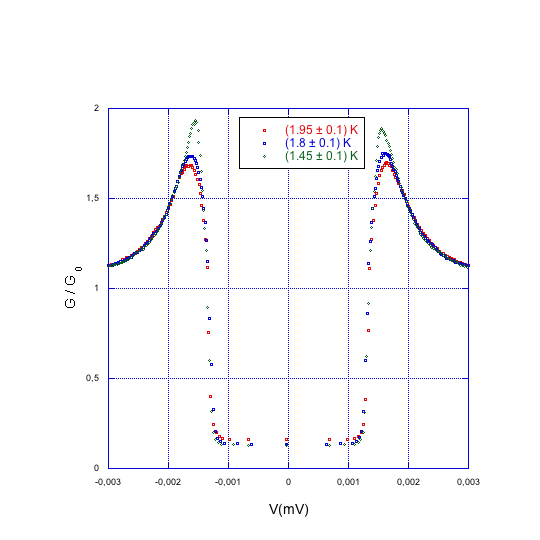
\includegraphics[scale=0.4]{graph1}
\caption{Hola\label{graph1}}
\end{figure}

\begin{figure}[h!]
\centering
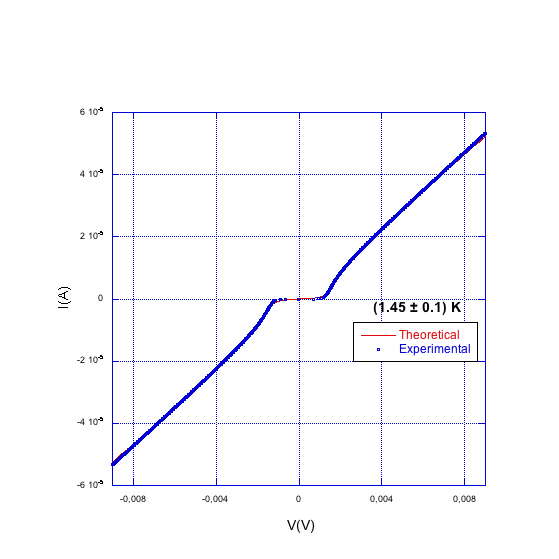
\includegraphics[scale=0.4]{graph2}
\caption{Hola\label{graph2}}
\end{figure}

\begin{figure}[h!]
\centering
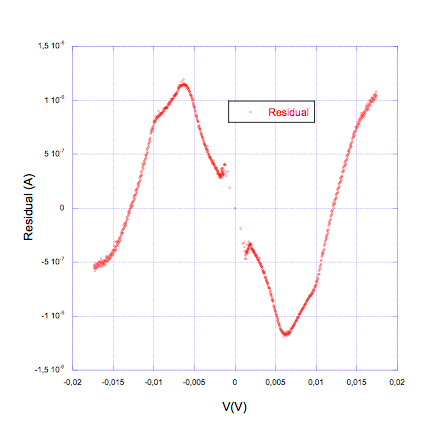
\includegraphics[scale=0.4]{graph3}
\caption{Hola\label{graph3}}
\end{figure}

\begin{figure}[h!]
\centering
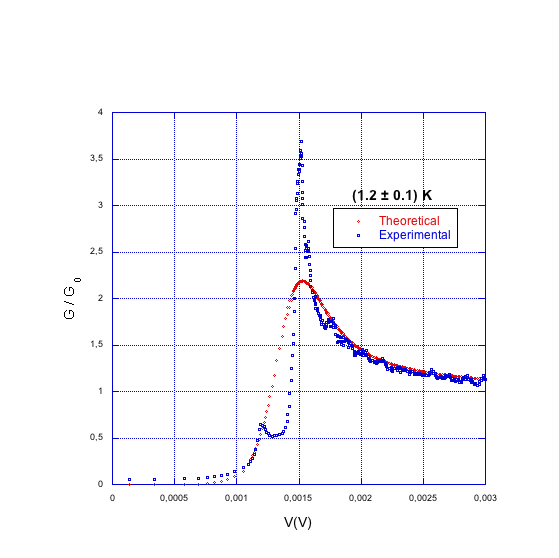
\includegraphics[scale=0.4]{graph4}
\caption{Hola\label{graph4}}
\end{figure}

\begin{figure}[h!]
\centering
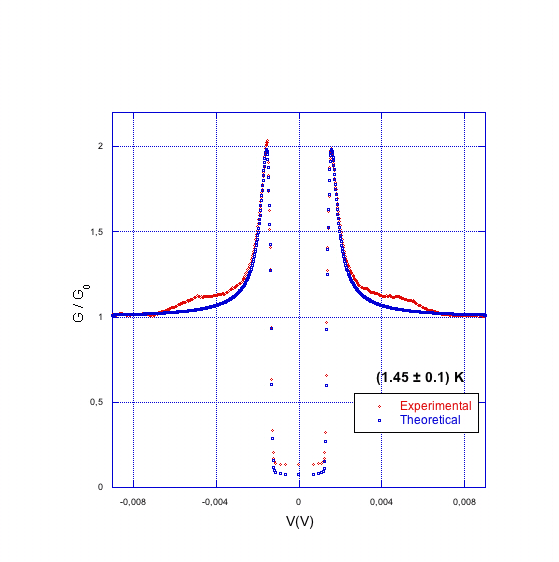
\includegraphics[scale=0.4]{graph5}
\caption{Hola\label{graph5}}
\end{figure}



%-----------------------------------------------------------------
%-----------------------------------------------------------------
\section{Results and Analysis}

1) Levenberg-Marquard??? The best method: by hand... :-)
2) Graphs: commentary on ALL the characteristics...
3) BCS is not totally correct --> real density of states is not the BCS's one, phonons,
4) ...


These are the Experimental ResultsThese are the Experimental Results These are the Experimental Results These are the Experimental Results These are the Experimental Results These are the Experimental Results These are the Experimental Results These are the Experimental Results These are the Experimental Results These are the Experimental Results These are the Experimental Results These are the Experimental Results These are the Experimental Results These are the Experimental Results These are the Experimental Results These are the Experimental Results These are the Experimental Results These are the Experimental Results These are the Experimental Results These are the Experimental Results These are the Experimental Results 


%-----------------------------------------------------------------
%-----------------------------------------------------------------
%-----------------------------------------------------------------
%-----------------------------------------------------------------
\begin{thebibliography}{99}

\bibitem{giaever1} I. Giaever and K. Megerle, \emph{Study of Superconductors by Electron Tunneling}, Phys. Rev. vol. 122, Num. 4, p. 1101 (1961)

\bibitem{giaever2} I. Giaever, \emph{Electron Tunneling and Superconductivity}, Rev. Mod. Phys. vol. 48, Num. 2, (1974)

\bibitem{giaever3} I. Giaever, \emph{Energy Gap in Superconductor Measured by Electron Tunneling}, Phys. Rev. Let. vol. 5, Num. 4, p. 147 (1960)

\bibitem{frerichs} R. Frerichs and J. P. Wilson, \emph{Tunnel-Effect Measurements on Superimposed Layers of Lead and Aluminum}, Phys. Rev. vol. 142, Num. 1, p. 264 (1966)

\bibitem{bcs} J. Bardeen, L. N. Cooper and J. R. Schrieffer, \emph{Theory of Superconductivity}, Phys. Rev. vol. 108, Num. 5, p. 1175 (1957)

\bibitem{ashcroft} N. W. Ashcroft and N. D. Mermin, \emph{Solid State Physics}, Harcourt College Publishers (1976)

\bibitem{formulas} Jianping Li, \emph{General explicit difference formulas for numerical differentiation}, Journal of Computational and Applied Mathematics vol. 183, p. 29 (2005)

\bibitem{recipes} W. H. Press, S. A. Teukolsky, W. T. Vetterling and B. P. Flannery \emph{Numerical Recipes},  Cambridge University Press (1997)



\end{thebibliography}

%-----------------------------------------------------------------
%-----------------------------------------------------------------
%-----------------------------------------------------------------
%-----------------------------------------------------------------
\end{document}